\documentclass[12pt]{article}
\usepackage{amsmath, amssymb, amsthm}
\usepackage{geometry}
\usepackage{xcolor}
\usepackage{graphicx}
\geometry{margin=1in}

\title{Engineering Probability \\ Homework 3}
\author{Timothy Pollard, pollat@rpi.edu}
\date{September 22th 2025}

\begin{document}

\maketitle
\hrulefill

\section*{(1)}
The random variable V has PMF.
\[
P_V(v) =
\begin{cases}
cv^2, & v = 1,2,3,4, \\
0, & \text{otherwise}.
\end{cases}
\]

\begin{enumerate}
    \item[(a)] Find the value of the constant c. \textcolor{blue}{\[1=c(1)^2+c(2)^2+c(3)^2+c(4)^2 \] \[1=30c \implies \frac{1}{30}=c\]}
    \item[(b)] Find $P\left[V \in \{u^2 \mid u = 1,2,3,\dots \}\right]$. \textcolor{blue}{\[P(V_{Square}) =c(1)^2 +c(4)^2\] \[P(V_{square}) =\frac{1}{30}(1)^2 +\frac{1}{30}(4)^2=\frac{17}{30}\]}
    \item[(c)] Find the probability that $V$ is an even number. \textcolor{blue}{\[P(V_{Even}) = c(2)^2+c(4)^2\] \[P(V_{Even}) = \frac{1}{30}(2)^2+\frac{1}{30}(4)^2 = \frac{20}{30} =\frac{2}{3}\]}
    \item[(d)] Find $P[V\ge 2]$.  \textcolor{blue}{\[P(V\geq 2) = c(2)^2+c(3)^2+c(4)^2\] \[P(V\geq 2) = \frac{1}{30}(2)^2+\frac{1}{30}(3)^2+\frac{1}{30}(4)^2 = \frac{29}{30}\]}
\end{enumerate}

\section*{(2)}
When someone presses “SEND” on a cellular phone, the phone attempts to set
up a call by transmitting a “SETUP” message to a nearby base station. The phone waits
for a response and if none arrives within 0.5 seconds it retries again. If it doesn’t get a
response after $n = 6$ tries, the phone stops transmitting messages and generates a busy
signal.

\begin{enumerate}
    \item[(a)] Draw a tree diagram that describes the call set-up procedure.
    \item[] \centering 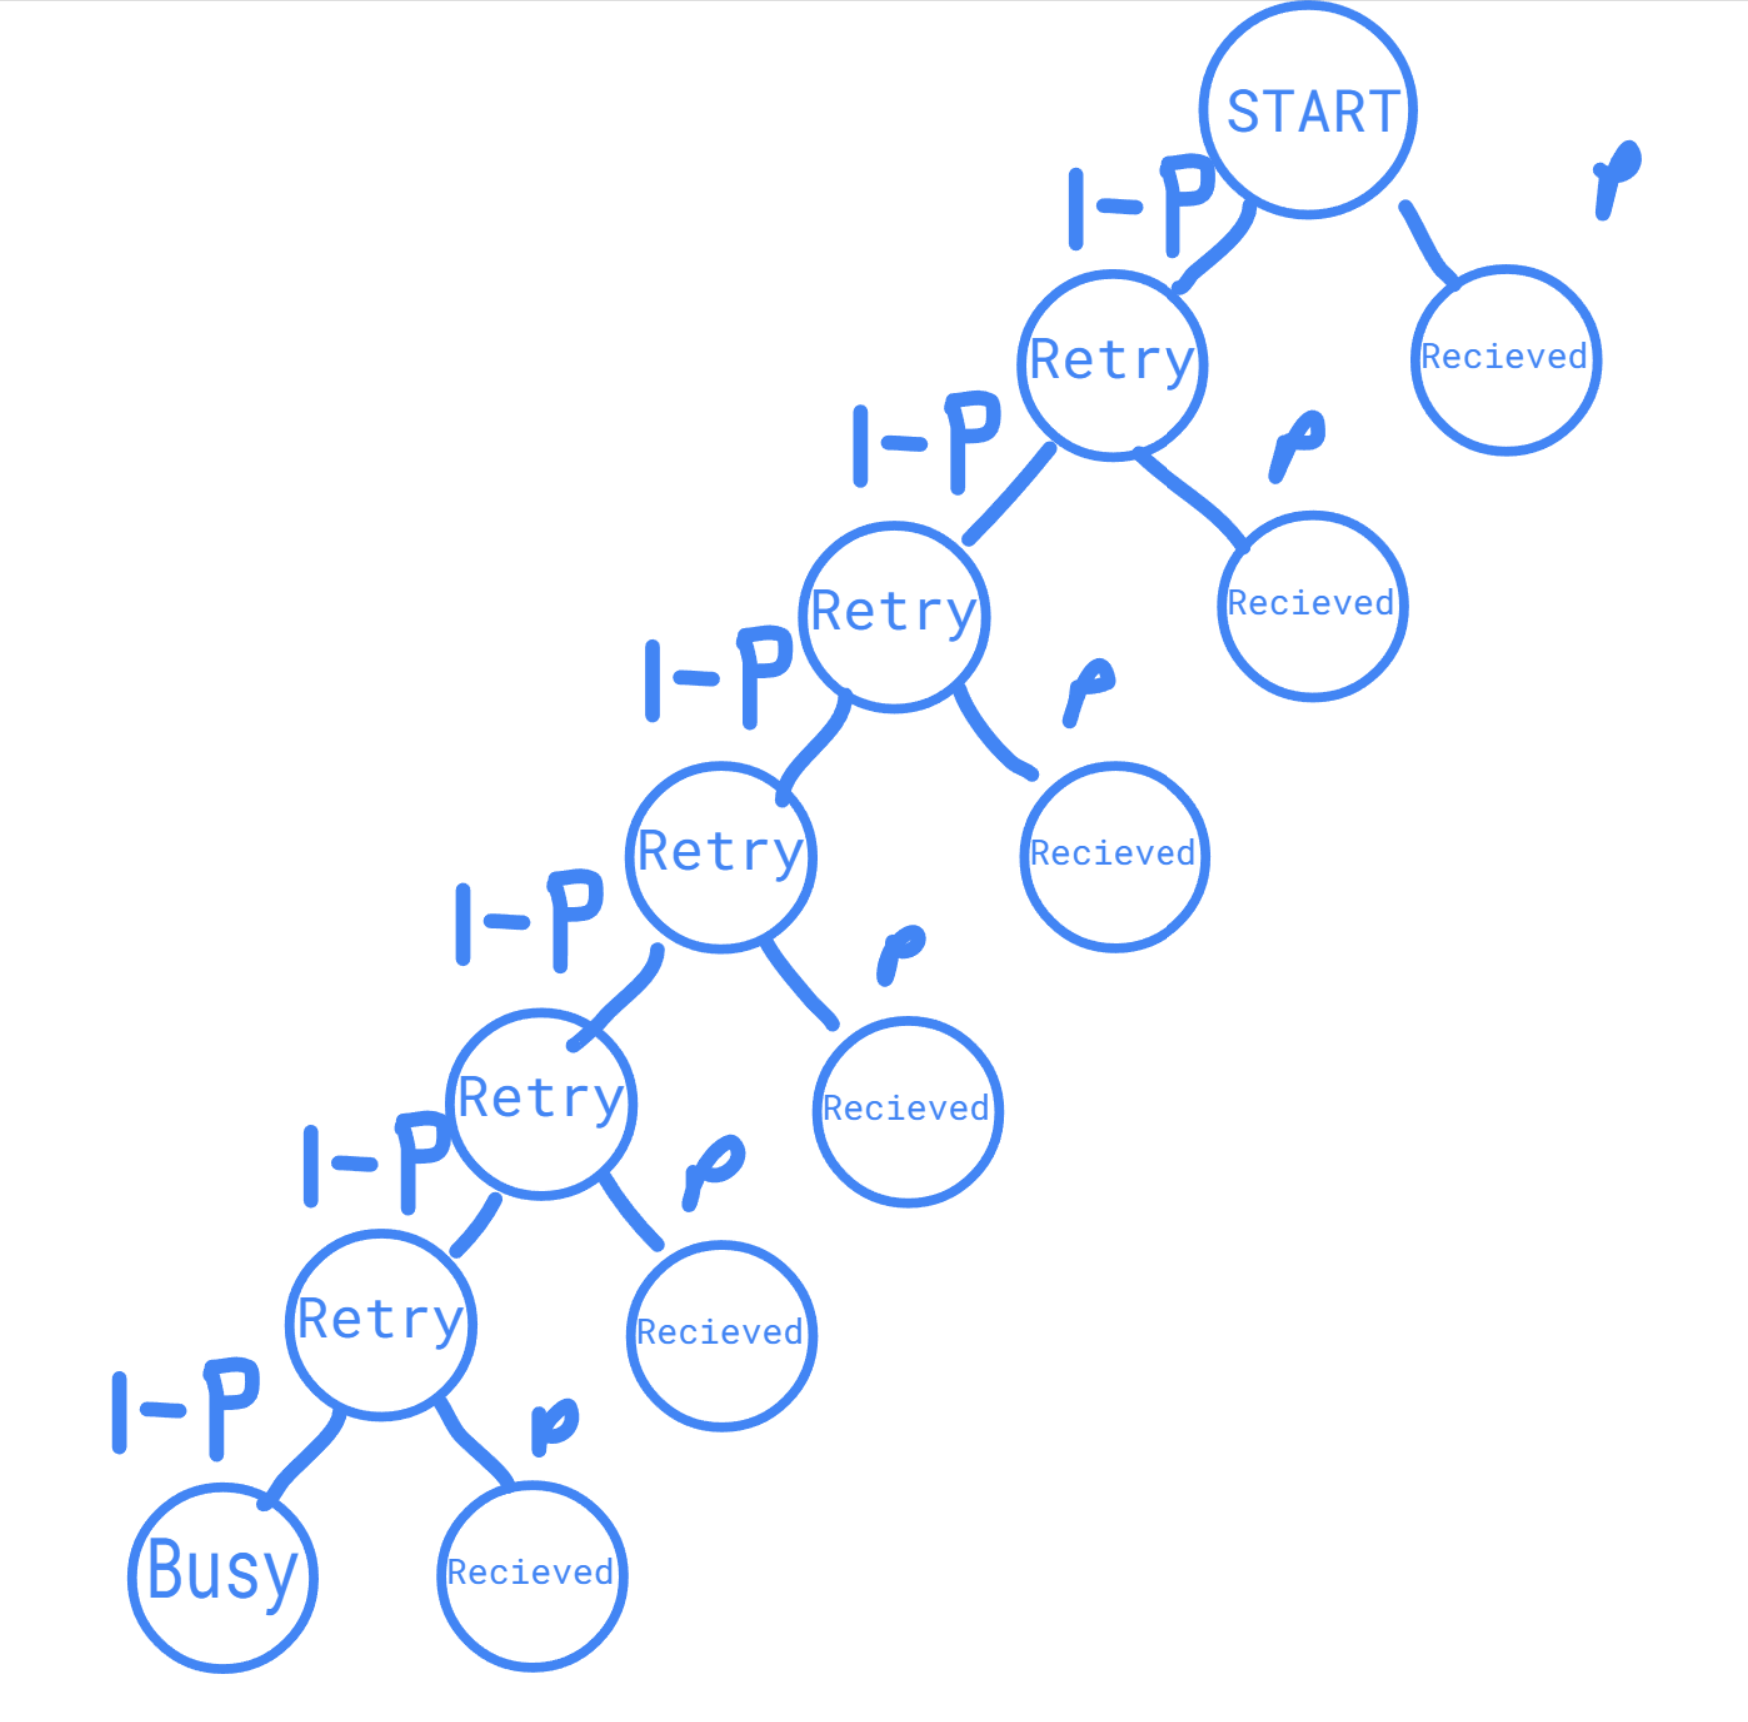
\includegraphics[width=0.4\textwidth]{Screenshot 2025-09-20 185143.png}
    \item[(b)] If all transmissions are independent and the probability is $p$ that a ``SETUP'' message will get through, what is the PMF of $K$, the number of messages transmitted in a call attempt?
    \item[] \textcolor{blue}{\[P_K(k)=
\begin{cases}
p(1-p)^{1-k}, & k = 1,2,3... n-1 \\
(1-p)^n, & k=n.
\end{cases}
\]}
    \item[(c)] What is the probability that the phone will generate a busy signal?
    \item[] \textcolor{blue}{$(1-p)^n =(1-p)^6$}
    \item[(d)] As manager of a cellular phone system, you want the probability of a busy signal to
    be less than 0.02. If $p = 0.9$, what is the minimum value of $n$ necessary to achieve
    your goal?
    \textcolor{blue}{
    \[
    \begin{aligned}
        0.02&>(1-p)^n\\
        0.02&>(1-0.9)^n\\
        0.02&>(0.1)^n\\
        \log_{0.1}{0.02}&<n\\
        \log_{0.1}{0.02}&\approx1.699\\
        \text{min: }n=2 
    \end{aligned}
    \]
    }
\end{enumerate}
\newpage

\section*{(3)}
When a two-way paging system transmits a message, the probability that the
message will be received by the pager it is sent to is $p$. When the pager receives the
message, it transmits an acknowledgement signal (ACK) to the paging system. If the
paging system does not receive the ACK, it sends the message again.

\begin{enumerate}
    \item[(a)] What is the PMF of $N$, the number of times the system sends the same message?
    \item[] \textcolor{blue}{\[
P_N(n) =
\begin{cases}
p(1-p)^{n-1}, & n = 1,2,3,4,\cdots \\
0, & \text{otherwise}.
\end{cases}
\]}
    \item[(b)] The paging company wants to limit the number of times it has to send the same
    message. It has a goal of $P[N \leq 3] \geq 0.95$. What is the minimum value of $p$ necessary to achieve the goal?
    \item[] 
\textcolor{blue}{
\[
\begin{aligned}
P[N \leq 3] &= P(N = 1) + P(N = 2) + P(N = 3) \\
P[N \leq 3] &= p(1 - p)^{0} + p(1 - p)^{1} + p(1 - p)^{2} \\
P[N \leq 3] &= p + p(1 - p) + p(1 - p)^2 \\
P[N \leq 3] &= p + (p - p^2) + (p - 2p^2 + p^3) \\
P[N \leq 3] &= 3p - 3p^2 + p^3 \\
0.95 &= 3p - 3p^2 + p^3 \\
p &\approx 0.6316 \\
\end{aligned}
\]
}
\end{enumerate}
\newpage
    
\section*{(4)}
 A radio station gives a pair of concert tickets to the sixth caller who knows the
birthday of the performer. For each person who calls, the probability is 0.75 of knowing
the performer’s birthday. All calls are independent.

\begin{enumerate}
    \item[(a)] What is the PMF of $L$, the number of calls necessary to find the winner?
    \item[] \textcolor{blue}{\[
P_L(l) =
\begin{cases}
\binom{l-1}{5}(0.75)^6(1-0.75)^{l-6}, & l = 6,7,8 \cdots, l=6+k | k\in \mathbb{N} \\
0, & \text{otherwise}.
\end{cases}
\]}
    \item[(b)] What is the probability of finding the winner on the tenth call?
    \item[] \textcolor{blue}{\[P_L(10) = \binom{(10)-1}{5}(0.75)^6(1-0.75)^{(10)-6} \approx 0.1752\]}
    \item[(c)] What is the probability that the station will need nine or more calls to find a winner?
    \textcolor{blue}{\[
    \begin{aligned}
    P_L(L\geq 9) &= (1-P_L(L < 9)) = (1-(P_L(6)+P_L(7)+P_L(8)))\\
    P_L(L\geq 9) &= 1-\left(\binom{5}{5}(0.75)^6(0.25)^{(6)-6}+\binom{6}{5}(0.75)^6(0.25)^{(7)-6}+\binom{7}{5}(0.75)^6(0.25)^{(8)-6}\right)\\
    P_L(L\geq 9) & \approx 0.3215\\
    \end{aligned}\]}
\end{enumerate}

\section*{(5)}
A certain phone-sensor fails to activate if it receives fewer than four photons in a
certain time interval. If the number of photons is modelled by a Poisson random variable
$X$ with $\alpha = 2$, find the probability that the sensor activates.

\textcolor{blue}{\[
P_X(x) =
\begin{cases}
\frac{(2)^x e^{-(2)}}{x!}, & x = 1,2,3 \cdots \\
0, & \text{otherwise}.
\end{cases}
\]
\[
\begin{aligned}
P_X(x\geq 5)&= 1 - P_X(x < 5)\\
P_X(x\geq 5)&= 1- \left(P_X(1)+P_X(2)+P_X(3)+P_X(4)+P_X(5)\right)\\
P_X(x\geq 5)&=  1- \left(\frac{(2)^{(1)} e^{-2}}{(1)!}+\frac{(2)^{(2)} e^{-2}}{(2)!}+\frac{(2)^{(3)} e^{-2}}{(3)!}+\frac{(2)^{(4)} e^{-2}}{(4)!}+\frac{(2)^{(5)} e^{-2}}{(5)!}\right)\\
P_X(x\geq 5)&=  1- e^{-2}\left(\frac{(2)^{(1)}}{(1)!}+\frac{(2)^{(2)} }{(2)!}+\frac{(2)^{(3)} }{(3)!}+\frac{(2)^{(4)} }{(4)!}+\frac{(2)^{(5)}}{(5)!}\right)\\
P_X(x\geq 5)&=  1- e^{-2}\left(2+2+\frac{8}{6}+\frac{16}{24}+\frac{32}{120}\right)\\
P_X(x\geq 5)&\approx 0.1519  \\
\end{aligned}
\]
}
\end{document}

